\documentclass[urlcolor=blue,dvipsnames]{beamer}

\usepackage[utf8]{inputenc}
\usepackage{fancybox,fancyvrb}
\usepackage{environ,xspace,empheq}

\usepackage{tikz}
\usetikzlibrary{arrows.meta,decorations.markings,decorations.pathreplacing,fadings,positioning}

\hypersetup{colorlinks,linkcolor=,urlcolor=cyan}

\beamertemplatenavigationsymbolsempty
\setbeamertemplate{footline}[frame number]
\usetheme{Pittsburgh}

%\makeatletter
%\newcommand{\tinytiny}{\@setfontsize{\tinytiny}{4pt}{4pt}}
%\makeatother

\newcommand\enumnum[1]{{\renewcommand{\insertenumlabel}{#1}%
      \usebeamertemplate{enumerate item} \,}}

\newcommand{\grad}{\nabla}
\newcommand{\ih}{\boldsymbol{\hat{\textbf{\i}}}}
\newcommand{\jh}{\boldsymbol{\hat{\textbf{\j}}}}
\newcommand{\vF}{\boldsymbol{\vec{\textbf{F}}}}
\newcommand{\Matlab}{\textsc{Matlab}\xspace}
\newcommand{\Octave}{\textsc{Octave}\xspace}


\title{7.3 Laplace Transforms: \\ translations \& unit step functions}

\subtitle{a lesson for MATH F302 Differential Equations}

\author{Ed Bueler, Dept.~of Mathematics and Statistics, UAF}

\date{\tiny \today}


\begin{document}
\setbeamertemplate{itemize item}{$\bullet$}
\setbeamertemplate{itemize subitem}{$\circ$}
\renewcommand{\thefootnote}{{\color{green} \arabic{footnote}}}

\begin{frame}
\titlepage

\centerline{\tiny for textbook: \, D. Zill, \emph{A First Course in Differential Equations with Modeling Applications}, 11th ed.}
%\color{green!40!blue}
\end{frame}

\newcommand{\LL}[1]{\mathcal{L}\left\{#1\right\}}
\newcommand{\LLi}[1]{\mathcal{L}^{-1}\left\{#1\right\}}


\begin{frame}{the Laplace transform strategy}

\begin{center}
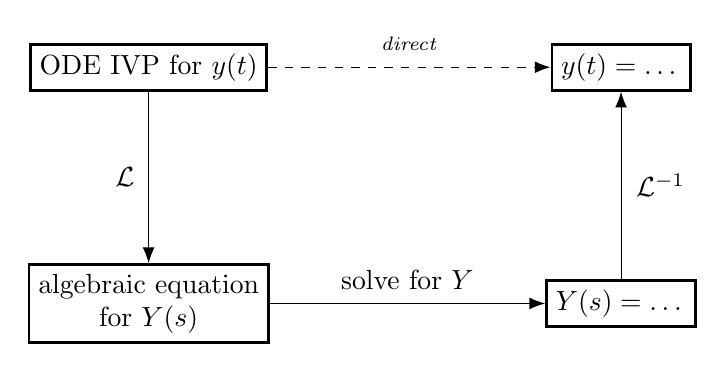
\begin{tikzpicture}[scale=1.0,>={Latex[length=2mm]},
  component/.style={rectangle,draw,fill=white,align=center,line width=1pt}]

\draw (-3,3) node[component] (ode) {ODE IVP for $y(t)$};
\draw (-3,0) node[component] (Leqn) {algebraic equation \\ for $Y(s)$};
\draw (3,0) node[component] (Lsoln)   {$Y(s)=\dots$};
\draw (3,3) node[component] (odesoln)   {$y(t)=\dots$};
\path
   (ode) edge[->] node[xshift=-3mm] {$\mathcal{L}$} (Leqn)
   (Leqn) edge[->] node[yshift=3mm] {solve for $Y$} (Lsoln)
   (Lsoln) edge[->] node[xshift=+5mm] {$\mathcal{L}^{-1}$} (odesoln)
   (ode) edge[dashed,->] node[yshift=3mm] {\scriptsize \emph{direct}} (odesoln);

\end{tikzpicture}
\end{center}

\begin{itemize}
\item \S 7.3: ``operational properties'' regarding translations (shifts)
    \begin{itemize}
    \item including the \emph{unit step function} $\mathcal{U}(t)$
    \item a.k.a.~\emph{Heaviside function}
    \end{itemize}
\item \S 7.4: ``operational property'' regarding \emph{convolution}
    \begin{itemize}
    \item in next slides
    \end{itemize}
\end{itemize}
\end{frame}


\begin{frame}{recall Laplace's Transform}

\begin{columns}
\begin{column}{0.77\textwidth}
\begin{itemize}
\item the definition:
    $$\LL{f(t)} = \int_0^\infty e^{-st} f(t)\,dt$$
\item first step is to apply $\mathcal{L}$ to ODE using
\begin{align*}
\LL{y'(t)} &= s Y(s) - y(0) \\
\LL{y''(t)} &= s^2 Y(s) - s y(0) - y'(0)
\end{align*}
\item doing $\mathcal{L}^{-1}$ is mostly use of a table, e.g.:
    \begin{itemize}
    \item $\displaystyle \LLi{\frac{1}{s-4}} = e^{4t}$
    \item $\displaystyle \LLi{\frac{k}{(s-a)^2+k^2}} = e^{at} \sin{kt}$
    \end{itemize}
\end{itemize}
\end{column}
\begin{column}{0.23\textwidth}
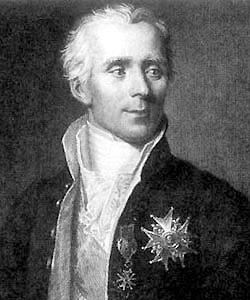
\includegraphics[width=\textwidth]{figs/Laplace-sharp}

\vspace{3mm}
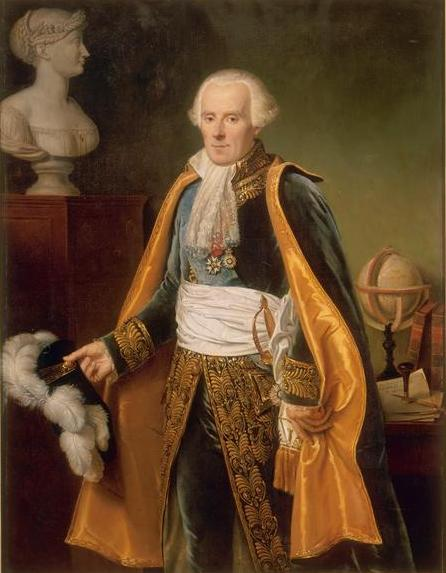
\includegraphics[width=\textwidth]{figs/Laplace-grand}

\tiny
Pierre-Simon Laplace (1749--1827) 
\end{column}
\end{columns}
\end{frame}


\begin{frame}{recall the better table}

\vspace{-2mm}
\begin{center}
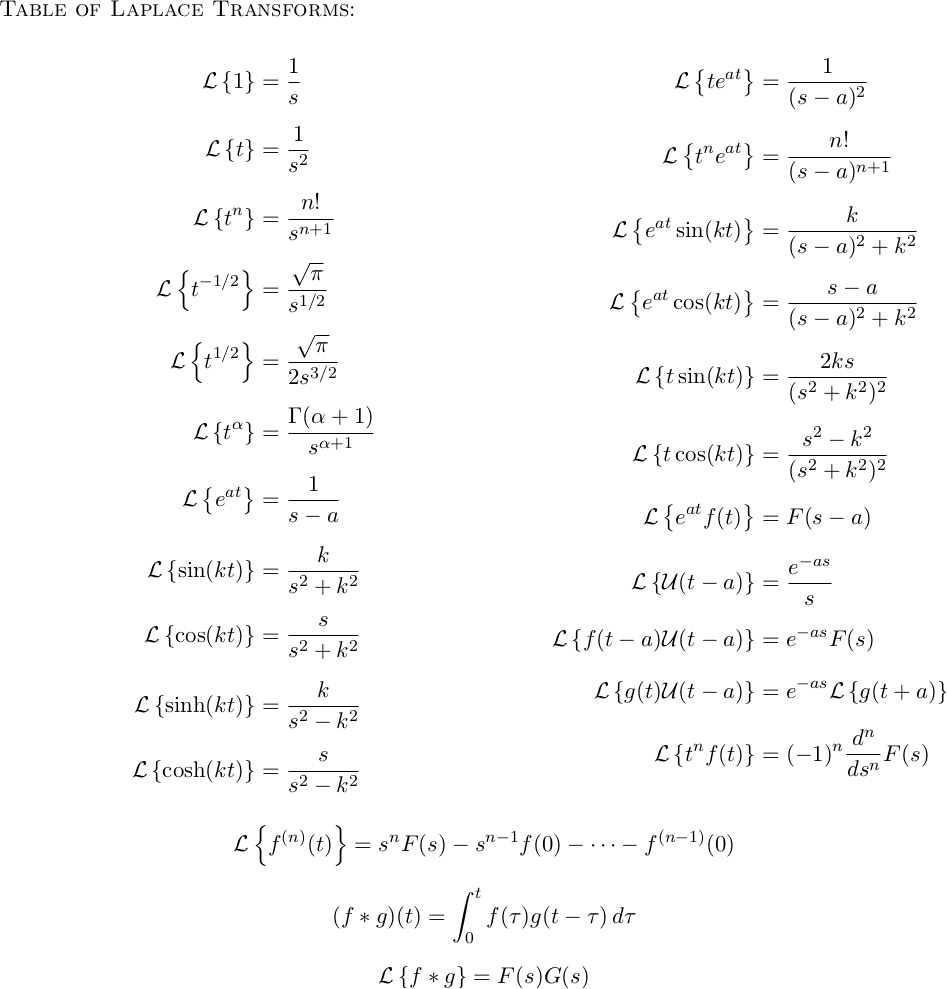
\includegraphics[height=80mm]{figs/fulllaplacetable}
\end{center}
\end{frame}


\begin{frame}{noticable in the table}

\begin{itemize}
\item compare the left and right columns in this part of the table:
\small
\begin{align*}
\LL{t} &= \frac{1}{s^2}            &&& \LL{te^{at}} &= \frac{1}{(s-a)^2} \\
\LL{t^n} &= \frac{n!}{s^{n+1}}     &&& \LL{t^n e^{at}} &= \frac{n!}{(s-a)^{n+1}} \\
\LL{\sin(kt)} &= \frac{k}{s^2+k^2} &&& \LL{e^{at}\sin(kt)} &= \frac{k}{(s-a)^2+k^2} \\
\LL{\cos(kt)} &= \frac{s}{s^2+k^2} &&& \LL{e^{at}\cos(kt)} &= \frac{s-a}{(s-a)^2+k^2}
\end{align*}
\item multiplying by $e^{at}$ causes: \, $s\to s-a$
\item this is indeed a rule!
\item multiplying by an exponential \emph{translates} the Laplace transform:
   $$\LL{e^{at} f(t)} = F(s-a)$$
\end{itemize}
\end{frame}


\begin{frame}{why?}

    $$\LL{e^{at} f(t)} = F(s-a)$$
\begin{itemize}
\item \alert{an exponential multiplier in $t$ is the same as a shift in $s$}
\item because, by definition,
\begin{align*}
\LL{e^{at} f(t)} &= \int_0^\infty e^{-st} e^{at} f(t)\,dt = \int_0^\infty e^{-(s-a)t} f(t)\,dt
\end{align*}
\end{itemize}
\end{frame}


\begin{frame}{examples}

\begin{itemize}
\item examples like in WebAssign 7.3
\item X
\end{itemize}
\end{frame}


\begin{frame}{X}

\begin{itemize}
\item X
\end{itemize}
\end{frame}


\begin{frame}{X}

\begin{itemize}
\item X
\end{itemize}
\end{frame}


\begin{frame}{X}

\begin{itemize}
\item X
\end{itemize}
\end{frame}


\begin{frame}{X}

\begin{columns}
\begin{column}{0.77\textwidth}
\begin{itemize}
\item X
\end{itemize}
\end{column}
\begin{column}{0.23\textwidth}
\vspace{3mm}

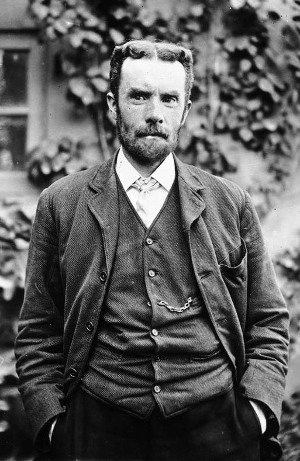
\includegraphics[width=\textwidth]{figs/Heaviside}

\tiny
Oliver Heaviside

(1850--1925)
\end{column}
\end{columns}
\end{frame}


\begin{frame}{summary}

\begin{itemize}
\item assume $\LL{f(t)}=F(s)$
\item \emph{1st translation theorem}.
    $$\LL{e^{at} f(t)} = F(s-a)$$
\item \emph{2nd translation theorem}.  if $a>0$ then
    $$\LL{f(t-a) \mathcal{U}(t-a)} = e^{-as} F(s)$$

\vspace{-2mm}
    \begin{itemize}
    \item includes easy-to-check case
    $$\LL{\mathcal{U}(t-a)} = \frac{e^{-as}}{s}$$
    \end{itemize}
\end{itemize}
\end{frame}


\begin{frame}{expectations}

\begin{itemize}
\item just watching this video is \emph{not} enough!
     \begin{itemize}
     \item see ``found online'' videos and stuff at

     \centerline{\href{https://bueler.github.io/math302/week11.html}{\tt \color{cyan} bueler.github.io/math302/week11.html}}
     \item \emph{read} sections 7.3 and 7.4 in the textbook
         \begin{itemize}
         \item but you can ignore ``beams'' in \S7.3, and
         \item you should focus on 7.4.2 Transforms of Integrals in \S7.4
         \end{itemize}
     \item \emph{do} the WebAssign exercises for section 7.3
         \begin{itemize}
         \item I will quiz on problems like these
         \end{itemize}
     \end{itemize}
\end{itemize}
\end{frame}

\end{document}

